% !TeX program = lualatex

\lecture{2}{2025-02-20}{Arithmetic Operations with integers}{}
\section{Addition of unsigned Integers}
\begin{parag}{By hand}
    We use here the same principle as a classical addition by hand of decimal numbers : 
\end{parag}
    \begin{center}
    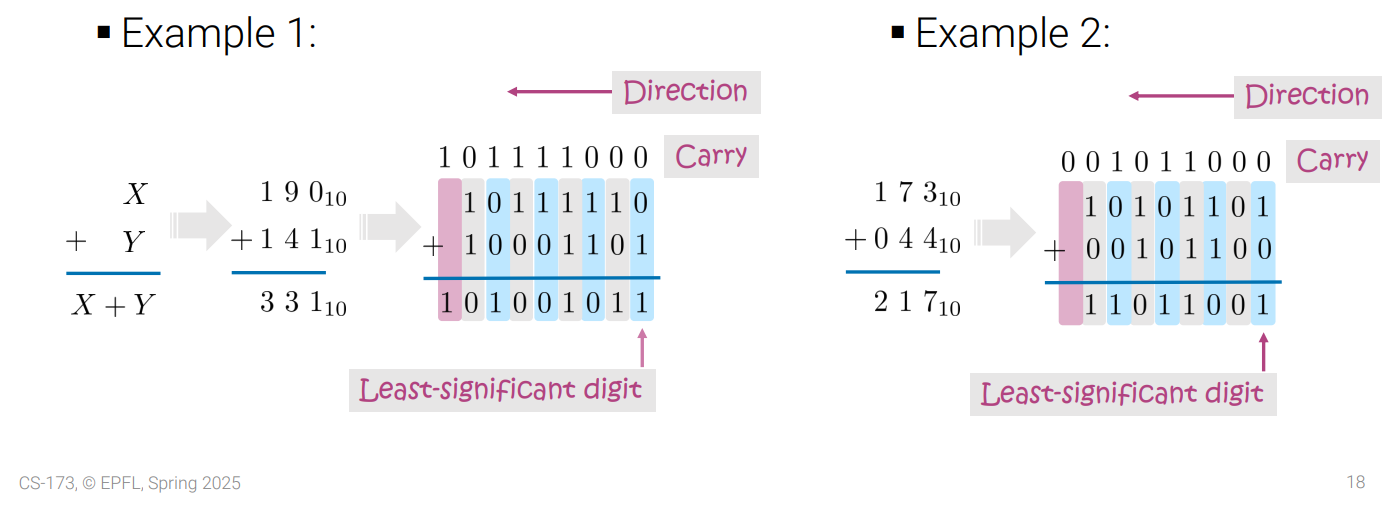
\includegraphics[scale=0.4]{Capture d’écran (112).png}
    \end{center}
\begin{parag}{How many Bits are needed}
    To represent the \important{sum of two $n$-bit unsigned numbers} we use \important{$n + 1$}
    \\
    For exemple the minimum space is when there are $0$ + $0$ which leads to : 
    \[s_{min} = 0 + 0 = 0\]
    and for the maximum : 
    \[s_{max} = (2^n - 1 ) + (2^n - 1) = 2\cdot 2^n -2 = 2^{n+1} - 2\]
    which makes it $n + 1$ bits for the sum.
    \begin{itemize}
        \item But we do not always have the extra bit in hardware
        \item When the magnitude of the result exceeds the largest representable value,  we say an \important{overflow} occurs and the result is incorrect.
    \end{itemize}
\end{parag}    
\subsection{Substraction of Unsigned Integers}
\begin{itemize}
    \item We use here the same idea as for decimal numbers : 
\end{itemize}
\begin{center}
    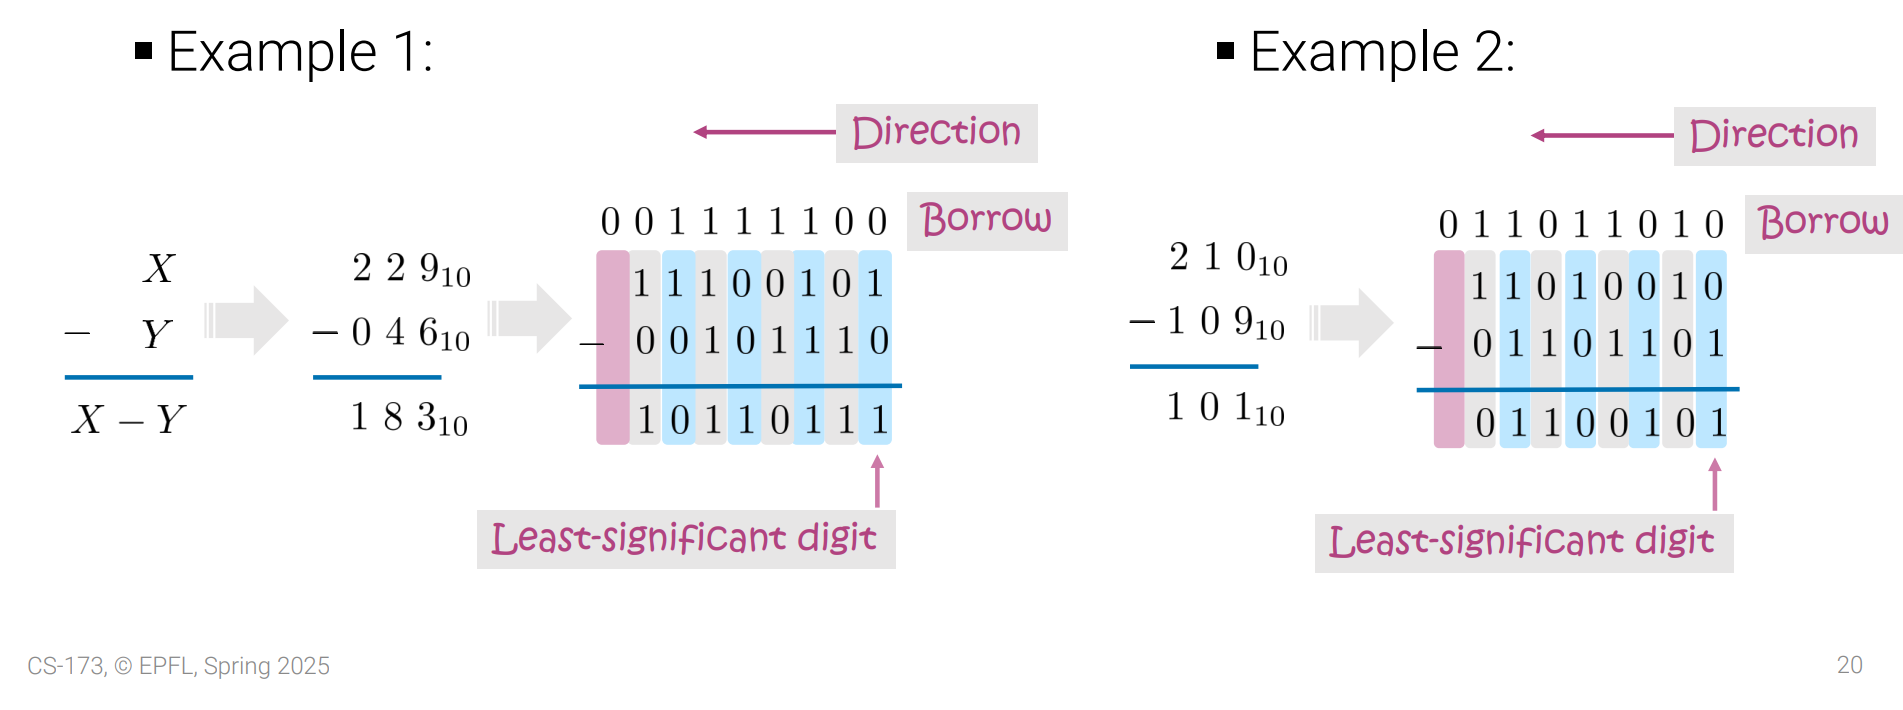
\includegraphics[scale=0.3]{Capture d’écran (113).png}
\end{center}
\begin{parag}{Negative result}
    \begin{itemize}
        \item Negative results cannot be represented using an unsigned system
        \item When trying to represent a value smaller than the minimu representable by the given number of bits $n$, an integer \important{underflow} occurs, and the result is incorrect.
    \end{itemize}
\end{parag}

\subsection{Two's Complement Addition/substraction}
\begin{parag}{Addition}
    We use here the same algorithm as for the unsigned numbers, and if the result exceeds the range, \important{overflow} occurs.
    \\
    To refresh how signes numbers works, for example $1000_2 = -8_{10}$ which is the "\textit{most negative}" number with $4$ bits. Then we add the right side of the number as positive integers like this:
    \[\underbrace{1}_{-8_{10}}\overbrace{010_2}^{2} = -6_{10}\]
    If we want to sum up $-5$ and $7$ for exemple:
    \begin{align*}
        1011 + 0111 \\
        \overbrace{1 + 1}^10\\
        \overbrace{1}^110 \\
        \overbrace{1}^1010 \\
        0010 = 2_{10}
    \end{align*}
    We use it as a clock : 
\end{parag}

\begin{center}
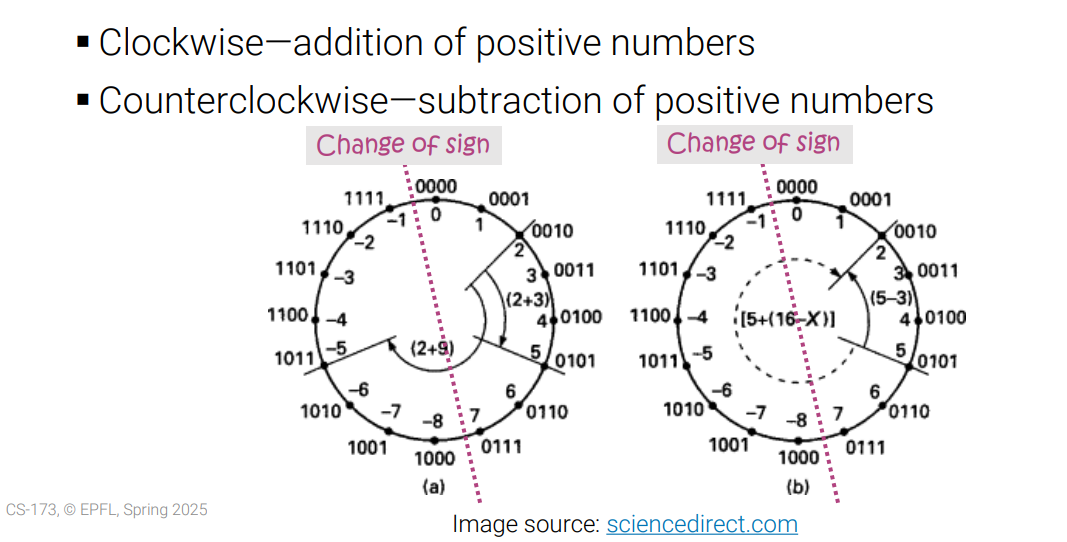
\includegraphics[scale=0.4]{Capture d’écran (114).png}
\end{center}

\begin{parag}{The preferred representation in digital Systems}
    \begin{itemize}
        \item If we start with the smallest (most negative) number $1000_2 = -8_{10}$ and count up all succesive numbers up to $0111_2 = 7_{10}$ can be obtained by adding $1$ to the previous one :
        \begin{itemize}
            \item The result will always be correct as long as the range is not exceeded
            \item Simple operation
            \item Not as simple for sign and magnitude
            \item Good for hardware implementation
            \begin{itemize}
                \item \important{Win-win}: the same hardware can perform the addition of unsigned numbers
            \end{itemize}
        \end{itemize}
    \end{itemize}
\end{parag}
\begin{parag}{Overflow Detection rules}
    \begin{itemize}
        \item Same algorithm as for the unsigned numbers
        \item If the result exceeds the range, \important{overflow} occurs
        \item \important{Overflow detection rules}
        \begin{itemize}
            \item If the signes of the two numbers are the same but different from the sign of the sum, the overflow occured
            \item Alternative formulation: if $c_{in}$ into  $c_{out}$ out of the sign position are different, the overflow occured
            \item Adding two numbers of different signs never produces an overflow
        \end{itemize}
    \end{itemize}
\end{parag}

\subsection{Binary multiplication}
\begin{parag}{How}
    We use the same "\textit{algorithm}" that the one we use by hand. For a binary representation:
    \begin{align*}
        X\cdot Y &= X \cdot \sum_{i=0}^{n-1} Y_i\cdot 2^i \\
        &= \sum_{i=0}^{n-1}X\cdot Y_i\cdot 2^i \\
        &= Y_{n-1} \cdot \underbrace{X \cdot 2^{n-1}}_{\text{Mulit Left-shifted by }n-1} + \cdots + Y_2\overbrace{X \cdot 2^2}^{\text{Mult Left shifted by }2} + Y_1\cdot X \cdot 2^1 + Y_0 \cdot X \cdot 2^0
    \end{align*}
\end{parag}
\begin{parag}{How many bits}
    \begin{theoreme}
        Given a $n$-bits intger and a $m$-bits intgers, there product can at most require $n + m$ bits.
    \end{theoreme}
    \begin{framedremark}
        We can see the multiplication as a sequence of $m$ additions with an $n$-bit number.
    \end{framedremark}
\end{parag}
\begin{parag}{Two's Complement multiplication}
    Recall of a value in two's complement (signed byte) : 
    \[x = -X_{n-1}2^{n-1} + \sum_{i = 0}^{n-2}X_i2^i\]
    \begin{itemize}
        \item Inspired by the previous algorithm:
        \begin{align*}
            X \cdot Y &= X \cdot (-Y_{n-1}\cdot 2^{n-1}) + X \sum_{i=0}^{n-2}Y_i\cdot 2^i \\
            &= -X\cdot Y_{n-1}\cdot 2^{n-1} + \sum_{i=0}^{n-2}X \cdot Y_i\cdot 2^i \\
            &= -Y_{n-1}\cdot X \cdot 2^{n-1} + Y_{n-2}\cdot X \cdot 2^{n-2} + \cdots + Y_2\cdot X\cdot 2^2 + Y_1\cdot X\cdot 2^1 + Y_0\cdot X\cdot 2^0
        \end{align*}
    \end{itemize}
    \begin{framedremark}
        Let us not forget the sign-extend the partial result
    \end{framedremark}
    For this only $n + m$ bits are kept; any higher-order bits are discarded. (that the "\textit{reason}" how $-5\cdot -3 = 15$
\end{parag}
\begin{parag}{Sign-Magnitude and Two's Complement}
    I juste want to underline the difference between those two representation. 
    \begin{subparag}{Sign Magnitude}
        In the Sign magnitude representation with $n$ bits, we use the \important{most significant bit} (MSB) to use it as a sign:
        \begin{itemize}
            \item $0$ for positive numbers
            \item $1$ for negative numbers
        \end{itemize}
        The remaining bits represent the absolute magnitude of the number:
        \\
        To write $5$ in a $4$-bits number, we use $0101_2 = +5_{10}$
        \\
        To write $-5$ in a $4$-bits number, we use $1101_2 = -5_{10}$
        \\
        We see here that it is very intuitive and mirrors human notation with a sign.
    \end{subparag}
    \begin{subparag}{Two's Complement Representation}
        Here, there is two point of view the one introduce in the course is to see it as a clock, in a clockwise (le sens des aiguilles d'une montre) it is positive, and unclockwise (dans le sens contraire à celui d'une montre) it is negative and begin. The negative also start at $-1$ but the bit to represent $-1$ is $1111_2$ which is just on the left.
        \\
        The other way is to see it as the most significant bit (MSB) as negative, $1000_2 = -8$ and the rest of the bits being positive. To write $-5$ you have to write it as $-8 + 3 = -5$ which goes to $1011_2 = -5_{10}$
        \\
        The pros for this notation is that there is only one representation for $0$ where there is two for the other ($1000 = 0000 = 0)$, The arithmetic operation are easier because we don't have to carry a sign everywhere and it is mor efficient in hardware implementation.
    \end{subparag}
\end{parag}    
\begin{figure}[h]
\centering
    \caption{Comparison table}
    \begin{tabular}{|c|c|c|}
    \hline
    Feature & Sign-Magnitude & Two's complement \\
    \hline
    \hline
     $-5_{10} $ & $1101$   &   $1011$ \\
     \hline
        Zero representation  & $0000 (+0)$ and $1000 (-0)$ & $0000$ \\
        \hline
        Range ($4$-bit) & $[-7, 7]$ & $[-8, +7]$ \\
        \hline
        
    \end{tabular}
    
    \label{fig:enter-label}
\end{figure}
    
    
